\section{Исходная задача}
Дан алгоритм, который производит релаксацию 3-хмерной матрицы. Каждая ячейка
на новой итерации релаксации вычисляется, как среднее арифметическое 6 ячеек,
которые ее окружают.
Т.е.
\begin{lstlisting}
A[i][j][k] = (A[i-1][j][k] + A[i+1][j][k] + A[i][j-1][k] + A[i][j+1][k] + A[i][j][k-1] + A[i][j][k+1]) / 6.}
\end{lstlisting}

Для решения данной задачи было решено разбивать исходный куб размера
$N \times N \times N$ на более мелкие части размера $m \times m \times m$,
где $m$ подбирается в зависимости от размера исходных данных.

Каждый MPI-процесс получает один или несколько кубов для обработки, после этого
передает граничные элементы в следующий процесс, который обрабатывает соседний
куб. Отдельно стоит рассмотреть граничные элементы, которые, вообще говоря,
могут иметь форму отличную от куба, если $m$ не является делителем $N$.

Приведем поясняющие схемы. На схеме \ref{fig:hyperplain} изображен куб для
исходной задачи без использования MPI. На схеме разными цветами выделены
диагональные плоскости куба. Заметим, что вычисление элементов такой плоскости
невозможно без вычисления элементов предыдущей плоскости.

\begin{figure}[H]
    \centering
    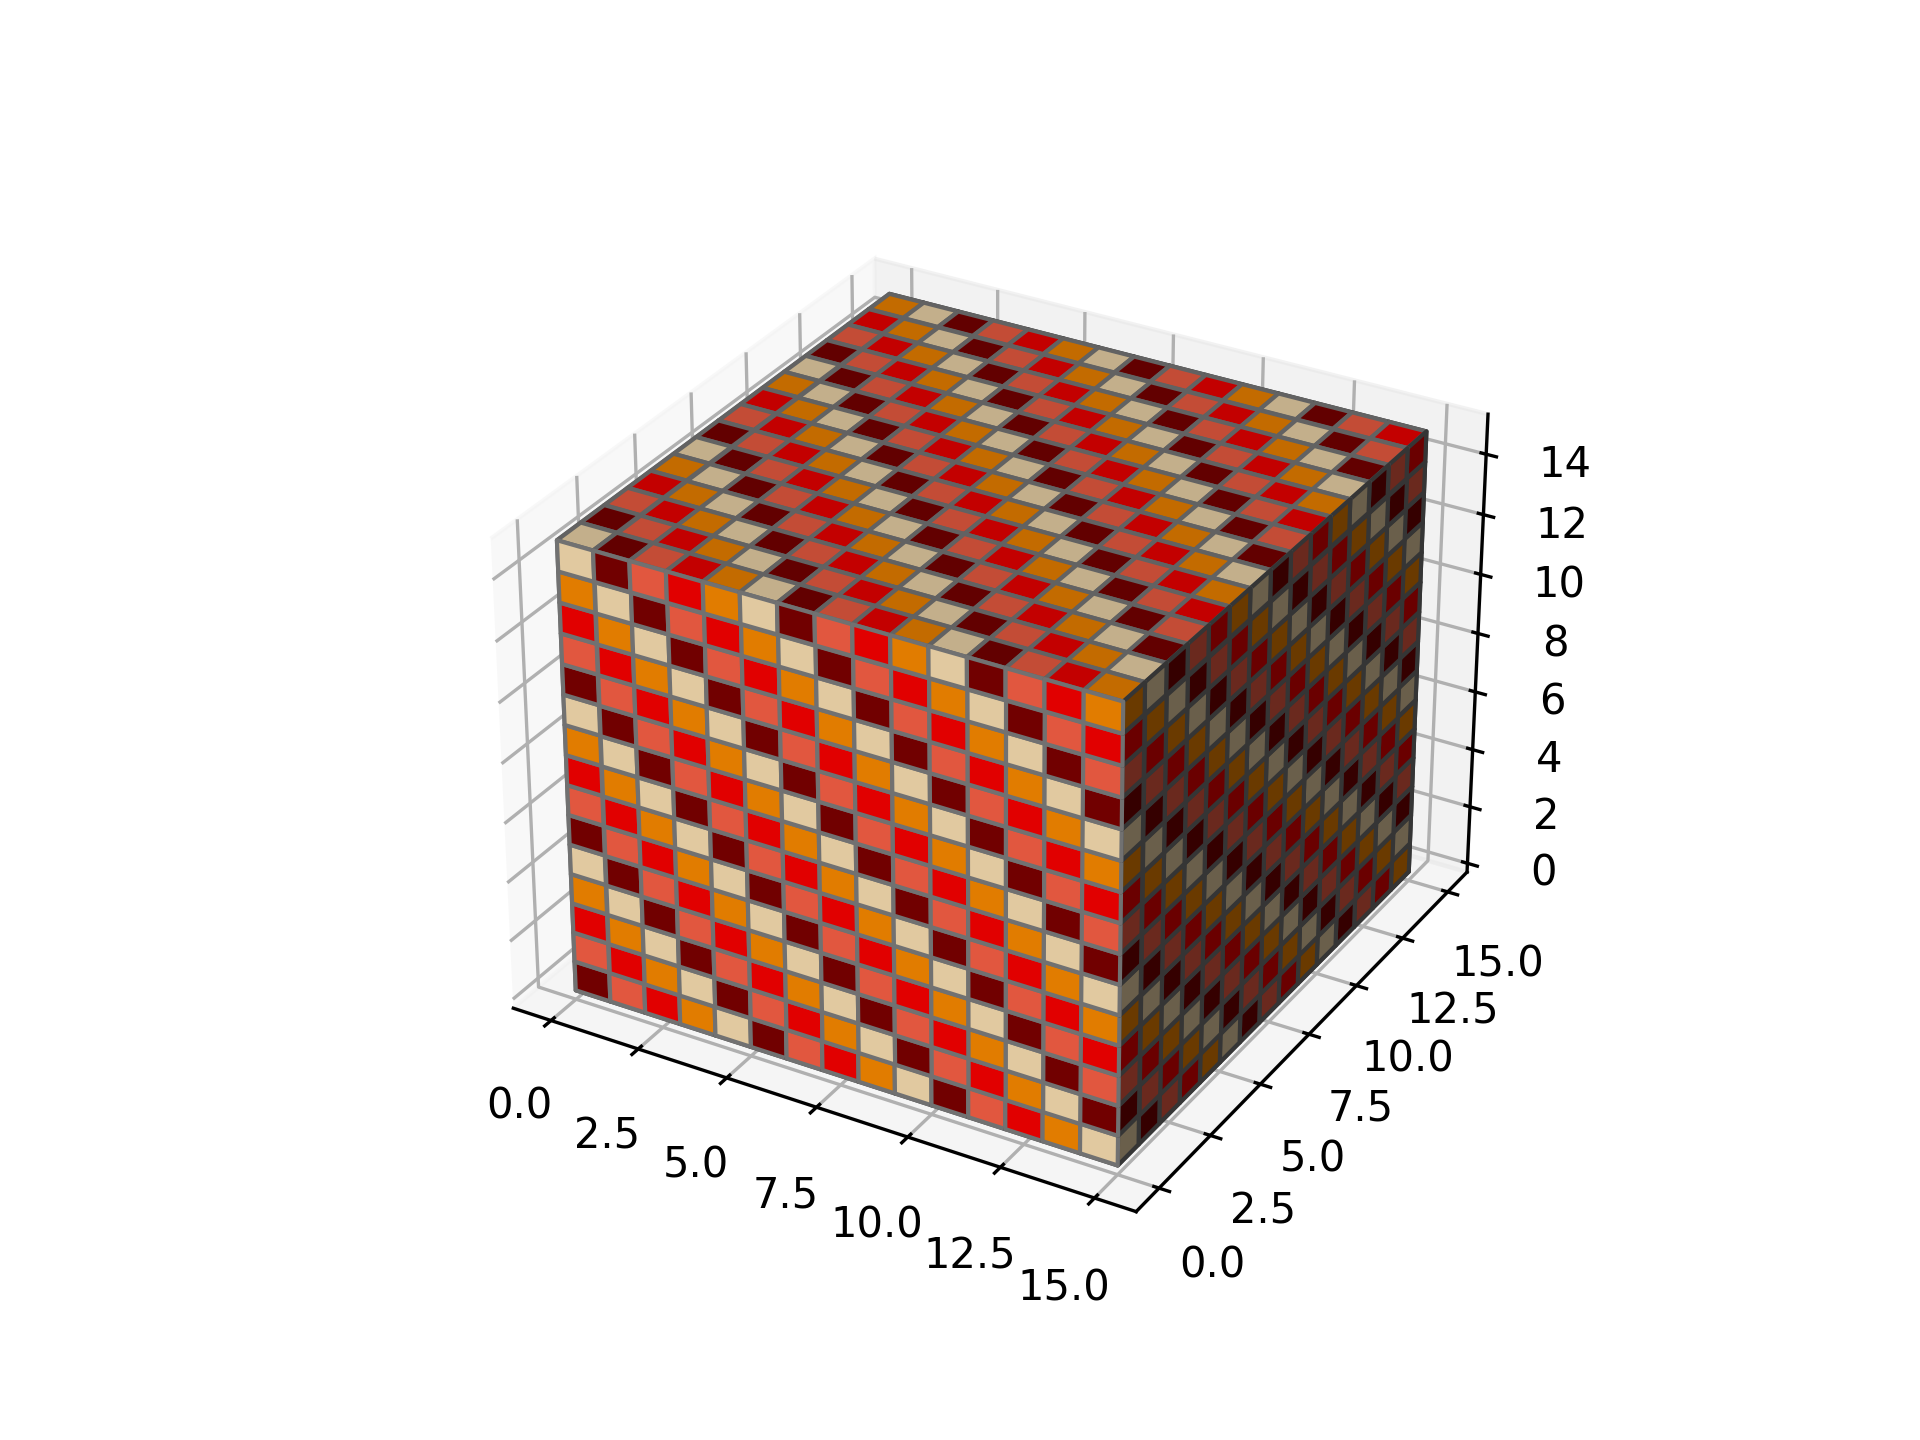
\includegraphics[width=1.\linewidth,center]{hyperplain.png}
    \caption{Схема работы алгоритма без использования MPI}
    \label{fig:hyperplain}
\end{figure}

Схема \ref{fig:big_hyperplain} иллюстрирует работу алгоритма с использованием
MPI. Куб был разбит на подкубы, и каждый малый куб будет вычисляться внутри
отдельного MPI-процесса. Каждый процесс может брать для вычисления несколько
независимых кубов.

\begin{figure}[H]
    \centering
    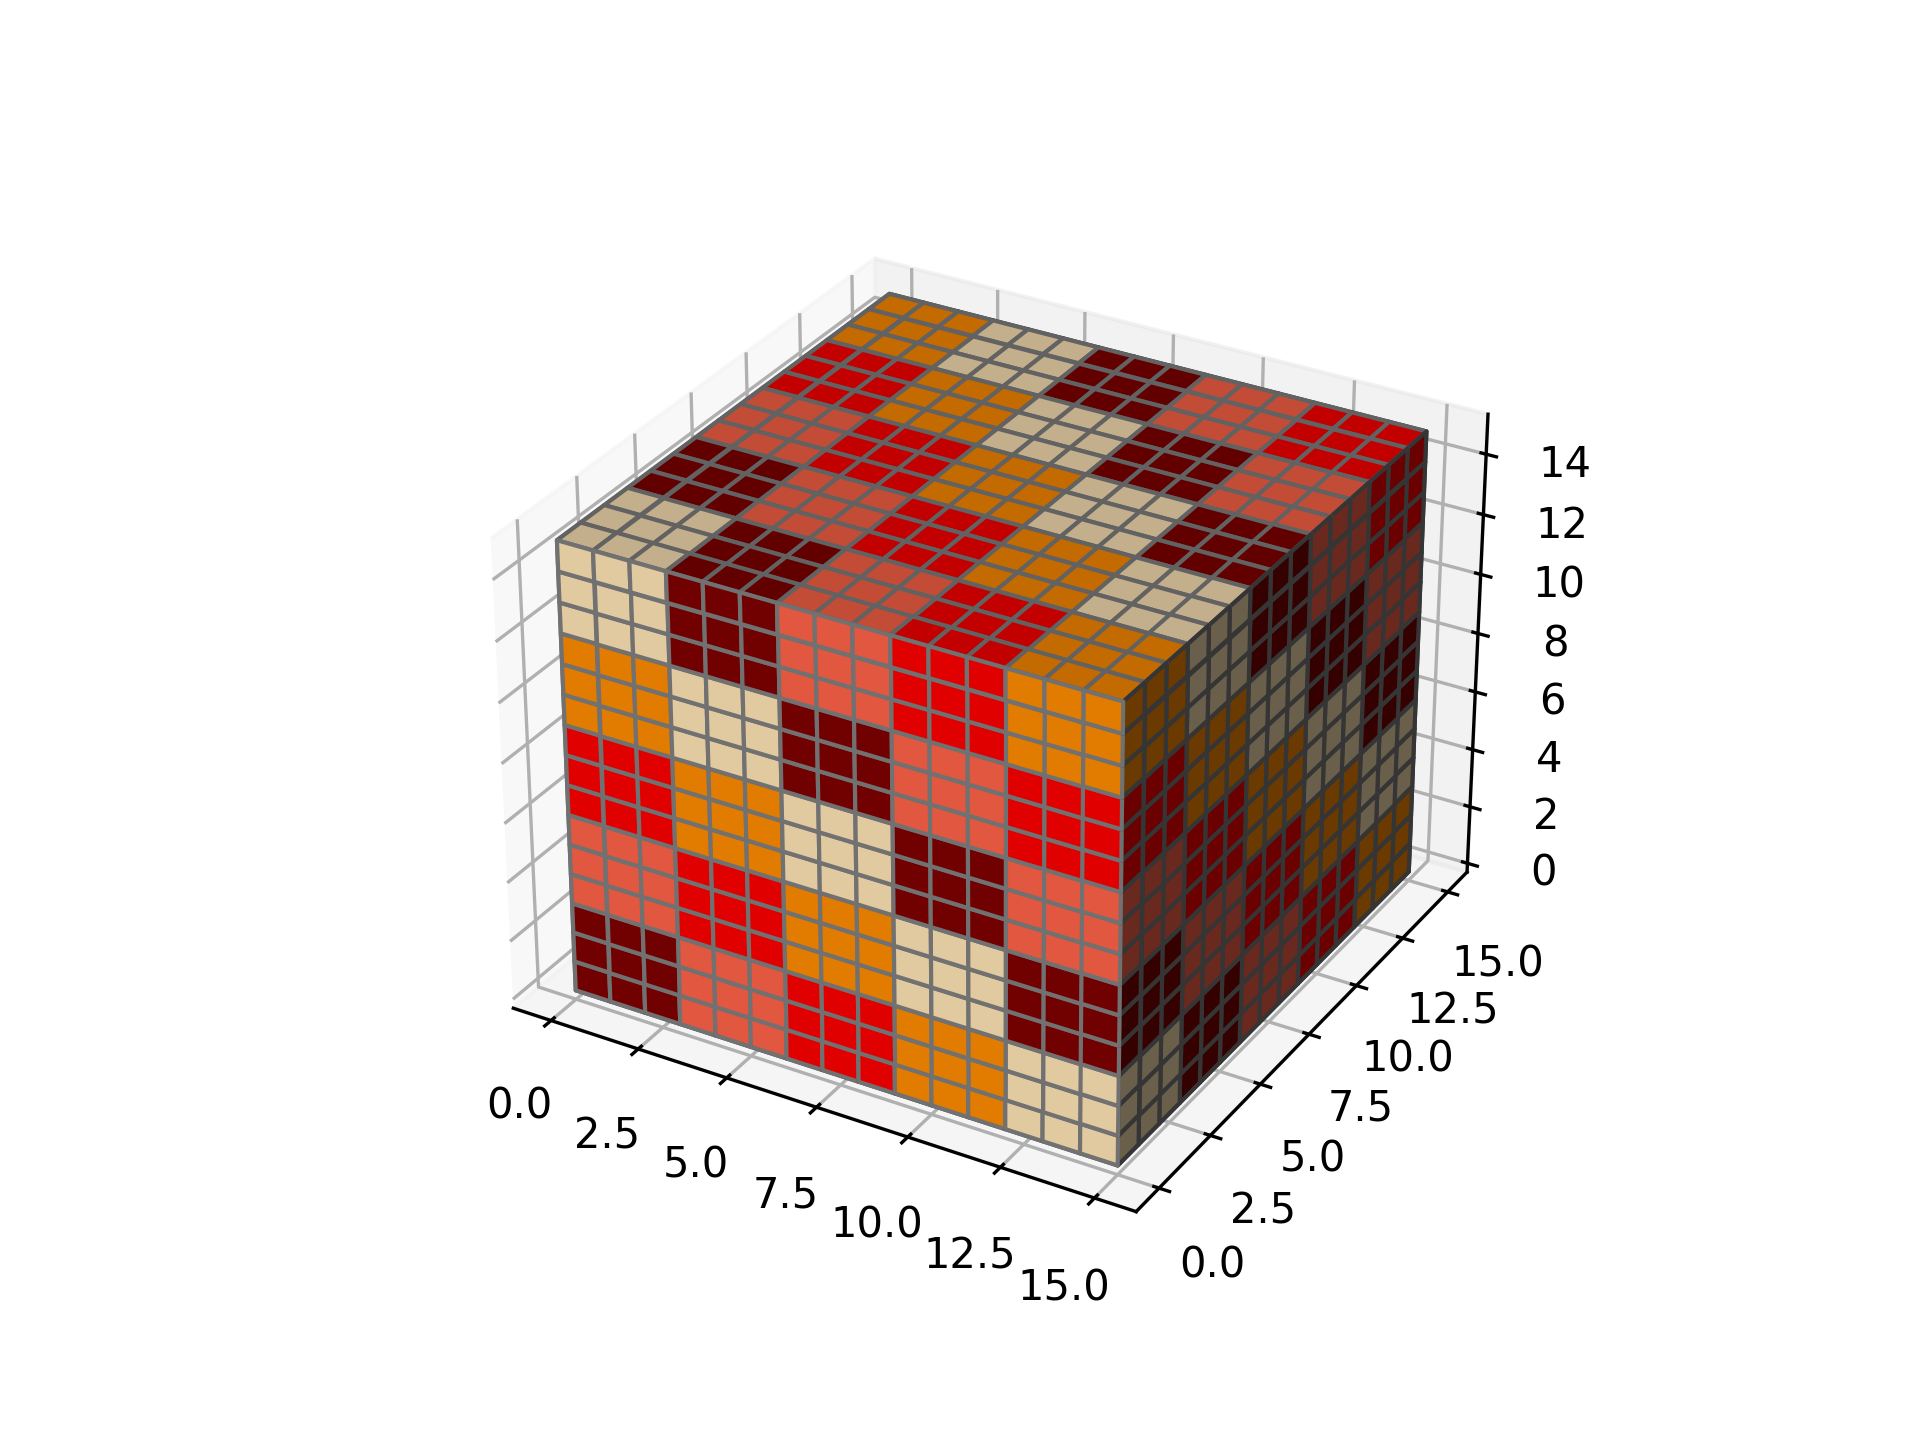
\includegraphics[width=1.\linewidth,center]{big_hyperplain.png}
    \caption{Схема работы алгоритма с использованием MPI}
    \label{fig:big_hyperplain}
\end{figure}

\section{Постановка задачи}
Доработать MPI-программу, реализованную в рамках курса <<Суперкомпьютеры и
параллельная обработка данных>>. Используя параллельный ввод-вывод (MPI-IO),
добавить контрольные точки для продолжения работы программы в случае сбоя.
Реализовать один из 3-х сценариев работы после сбоя: a) продолжить работу
программы только на <<исправных>> процессах; б) вместо процессов, вышедших из
строя, создать новые MPI-процессы, которые необходимо использовать для
продолжения расчетов; в) при запуске программы на счет сразу запустить
некоторое дополнительное количество MPI-процессов, которые использовать в
случае сбоя.

Для реализации был выбран сценарий В -- при запуске программы сразу запустить
некоторое дополнительное количество MPI-процессов, которые необходимо
использовать в случае сбоя.
